\section{Engineering aspects}\label{sec-engineering}

In the previous sections we have modelled the most critical subset of various
build systems. However, like all real-world systems, there are many corners that
obscure the essence. In this section we discuss some of those details, what
would need to be done to capture them in our model, and what the impact would be.

\subsection{Partial Stores and Exceptions}\label{sec-failures}

Our model assumes a world where the store is fully-defined, every \hs{k} is
associated with a \hs{v}, and every compute successfully completes returning a
valid value. In the real world, build systems frequently deal with errors, e.g.
``file not found'' or ``compilation failed''. We can model such failure
conditions by instantiating \hs{v} to either \hs{Maybe}~\hs{v} (for missing
values) or \hs{Either}~\hs{e}~\hs{v} (for exceptions of type \hs{e}). That can
model the errors inside the store and the \hs{Task}, but because our build
system models are polymorphic in \hs{v}, they cannot apply any special behaviour
for errors, e.g. aborting the build early. There are many other ways of
modelling errors, and in this section we show three simple examples.

As mentioned above, we can include failures into the type of values \hs{v}, for
example, to model a partial store we can use a simple like algebraic data type
isomorphic to \hs{Maybe}:

\vspace{1mm}
\begin{minted}[xleftmargin=10pt]{haskell}
data Value = FileNotFound | FileContents ByteString
\end{minted}
\vspace{1mm}

\noindent
This is convenient if \emph{tasks are aware of failures}. For example, a task
may be able to cope with missing files, e.g. if \hs{fetch}~\hs{"username.txt"}
returns \hs{FileNotFound}, the task could use the literal string \hs{"User"} as
a default value. In this case the task will \emph{depend} on the fact that the
file \cmd{username.txt} is missing, and will need to be rebuilt if the user
later creates this file. In general, we can use values of type
\hs{Either}~\hs{e}~\hs{v} when dealing with failures of type \hs{e}. To
automatically convert a ``failure-free'' task into an equivalent task operating
with values of type \hs{Either}~\hs{e}~\hs{v} we can use the following function:

\vspace{1mm}
\begin{minted}[xleftmargin=10pt]{haskell}
liftEither :: Task Monad k v -> Task Monad k (Either e v)
liftEither task = Task $ \fetch ->
    runExceptT $ run task (ExceptT . fetch)
\end{minted}
\vspace{1mm}

\noindent
Here \hs{liftEither} wraps the result of the given
\hs{fetch}~\hs{::}~\hs{k}~\hs{->}~\hs{Either}~\hs{e}~\hs{v} into \hs{EitherT}
and then runs the task in the \hs{EitherT} monad transformer~\cite{liang1995monad}.

Another approach is to include failures into the computation context \hs{f}. For
example, we can choose \hs{f}~\hs{=}~\hs{Maybe}:

\vspace{1mm}
\begin{minted}[xleftmargin=10pt]{haskell}
fetchA1A2 :: String -> Maybe Integer
fetchA1A2 k = Map.lookup k (Map.fromList [("A1", 10), ("A2", 20)])
\end{minted}
\vspace{1mm}

\noindent
Since tasks are polymorphic in \hs{f}, we can directly run them with the
callback \hs{fetchA1A2}. For example, the task \cmd{B1 = A1 + A2} from
\hs{sprsh1} in~\S\ref{sec-task} returns \hs{Just}~\hs{30}, whereas the task
\cmd{B2 = B1 * 2} returns \hs{Nothing} because \hs{fetchA1A2} fails on \cmd{B1}.

This approach is convenient if \emph{tasks are not aware of failures}, e.g. we
can model Excel formulas as pure arithmetic functions, and introduce failures
``for free'' if/when needed by instantiating \hs{Tasks} with an appropriate
\hs{f}.

Finally, the task itself might not want to encode failures into the type of
values \hs{v}, but instead \emph{demand that} \hs{f} \emph{has a built-in notion
of failures}. This can be done by choosing a suitable constraint \hs{c}, such as
\hs{Alternative}, \hs{MonadPlus} or even better something specific to failures,
such as \hs{MonadFail}. Then both the callback and the task can reuse the same
failure mechanism as shown below:

\vspace{1mm}
\begin{minted}[xleftmargin=10pt]{haskell}
class Monad m => MonadFail m where
    fail :: String -> m a

sprsh4 :: Tasks MonadFail String Integer
sprsh4 "B1" = Just $ Task $ \fetch -> do
    a1 <- fetch "A1"
    a2 <- fetch "A2"
    if a2 == 0 then fail "division by 0" else return (a1 `div` a2)
sprsh4 _ = Nothing
\end{minted}
\vspace{1mm}

\noindent
With this approach we can implement a build system that accepts
\hs{Tasks}~\hs{MonadFail}~\hs{k}~\hs{v} and handles errors by aborting the
build early and returning
\hs{Either}~\hs{String}~\hs{(Store}~\hs{i}~\hs{k}~\hs{v)} instead of just
\hs{Store}~\hs{i}~\hs{k}~\hs{v} as in~\S\ref{sec-general-build}. One possible
implementation is based on introducing an extra \hs{Either}~\hs{String} layer
into the monad stack; while fairly direct it is also tedious, and hence we omit
it.

% \todo{AM}{Add a MonadFail build system.}

\subsection{Parallelism}\label{sec-parallelism}

We have given simple implementations assuming a single thread of execution,
but all the build systems we address can actually build independent keys in
parallel. While it complicates the model, the complications can be restricted
exclusively to the scheduler:

\begin{enumerate}
\item The \hs{topological} scheduler can build the full dependency graph, and
whenever all dependencies of a task are complete, the task itself can be
started.

\item The \hs{restarting} scheduler can be made parallel in a few ways, but the
most direct is to have $n$ threads reading keys from the build queue. As before,
if a key requires a dependency not yet built, it is moved to the end~--~the
difference is that sometimes keys will be moved to the back of the queue not
because they are out of date but because of races with earlier tasks that had
not yet finished. As a consequence, if a the calculation order is persisted over
successive runs (as \Excel does), potentially racey dependencies will be
separated, giving better parallelism over time.

\item The \hs{suspending} scheduler can be made parallel by starting multiple
dependencies in parallel. One approach is to make the request for dependencies
take a list of keys, as implemented by \Shake. Another approach is to treat the
\hs{Applicative} dependencies of a \hs{Task}~\hs{Monad} in parallel, as
described by~Marlow~\etal~\shortcite{marlow2014haxl}.
\end{enumerate}

Once sufficient parallelism is available the next challenge is preventing excess
parallelism and machine resource starvation, which is usually achieved with a
thread pool or thread limit.

The actual implementation of the parallel schedulers is not overly onerous,
but neither is it beautiful or informative.


\subsection{Impure Computations}\label{sec-non-determinism}

In our model we define \hs{Task} as a function -- when given the same inputs
it will always produce the same output. Alas, the real-world is not so obliging.
Some examples of impure tasks include:

\begin{itemize}
\item \textbf{Untracked dependencies}: Some tasks depend on untracked values --
      for example C compilation will explicitly list the \cmd{source.c} file as
      a dependency, but it may not record that the version of \cmd{gcc} is also
      a dependency.

\item \textbf{Non-determinism}: Some tasks are \emph{non-deterministic},
      producing any result from a possible set. As an example, GHC programs
      compiled using parallelism can change the order in which unique variables
      are obtained from the supply, producing different but semantically
      identical results.

\item \textbf{Volatility}: Some tasks are defined to change in every build, e.g.
      \Excel provides a~``function'' \cmd{RANDBETWEEN} producing a fresh random
      number in a specified range on each recalculation. Similarly, build
      systems like \Make and \Shake provide volatile \emph{phony rules}. The
      main difference from non-deterministic tasks is that volatile tasks cannot
      be cached. They are best modelled as depending on a special key
      \cmd{RealWorld} whose value is changed in every build.
\end{itemize}

Interestingly, there is significant interplay between all three sources of
impurity. Systems like \Bazel use various sandboxing techniques to guard against
missing dependencies, but none are likely to capture all dependencies right down
to the CPU model and microcode version. Tasks that do have untracked
dependencies can be marked as volatile, a technique \Excel takes with the
\cmd{INDIRECT} function, removing the untracked dependency at the cost of
minimality.

Most of the implementations in \S\ref{sec-implementations} can deal with
non-determinism, apart from \Buck, which relies on deterministic tasks, and
in turn can optimise the number of roundtrips required to the server.

One tempting way of modelling non-determinism is to enrich \hs{Tasks} from
\hs{Applicative} or \hs{Monad} to \hs{Alternative} or \hs{MonadPlus},
respectively. Here is a task description corresponding to a spreadsheet with the
formula \cmd{B1 = A1 + RANDBETWEEN(1,2)}:

\begin{minted}[xleftmargin=10pt]{haskell}
sprsh3 :: Tasks MonadPlus String Integer
sprsh3 "B1" = Just $ Task $ \fetch -> (+) <$> fetch "A1"
                                          <*> (pure 1 <|> pure 2)
sprsh3 _    = Nothing
\end{minted}
\vspace{1mm}

\noindent
Such tasks can be modelled in our framework by adjusting the correctness
definition~(\S\ref{sec-build-correctness}), where instead of requiring that the
\hs{result}ing value \emph{equals} the one obtained by recomputing the \hs{task}:
\[
\hs{getValue}~\hs{k}~\hs{result}~\hs{==}~\hs{compute}~\hs{task}~\hs{result} %\text{,}
\]
\noindent
we now require that \hs{result} contains \emph{one possible result of
recomputing} the \hs{task}:
\[
\hs{getValue}~\hs{k}~\hs{result}~\hs{`elem`}~\hs{computeND}~\hs{task}~\hs{result} %\text{,}
\]
where
\hs{computeND}~\hs{::}~\hs{Task}~\hs{MonadPlus}~\hs{k}~\hs{v}~\hs{->}~\hs{Store}~\hs{i}~\hs{k}~\hs{v}~\hs{->}~\hs{[@@v]}
returns the list of all possible results of the \hs{task} instead of just one
value (`ND' stands for `non-deterministic').

% \todo{AM}{Show implementation of \hs{computeND}.
% Neil says: not convinced it's that interesting.}.

Note that \hs{Task}~\hs{MonadPlus} is powerful enough to model dependency-level
non-determinism, for example, \cmd{INDIRECT("A" \& RANDBETWEEN(1,2))}, whereas
most build tasks in real-life build systems only experience a value-level
non-determinism. \Excel handles this example simply by marking the cell
volatile~--~an approach that can be readily adopted by any of our
implementations.

\subsection{Cloud Implementation}\label{sec-cloud-aspects}

Our model of cloud builds provides a basic framework to discuss and reason
about them, but lacks a number of important engineering corners:

\begin{itemize}
\item \textbf{Communication}: When traces or contents are stored in the cloud,
communication can become a bottleneck, so it is important to send only the
minimum amount of information, optimising with respect to build system
invariants. For example, incremental data processing systems in the cloud, such
as \Reflow~\cite{reflow}, need to efficiently orchestrate terabytes of data.

\item \textbf{Offloading}: Once the cloud is storing build products and traces,
it is possible for the cloud to also contain dedicated workers that can execute
tasks remotely~--~offloading some of the computation and potentially running
vastly more commands in parallel.

\item \textbf{Eviction}: The cloud storage, as modelled
in~\S\ref{sec-constructive-traces}, grows indefinitely, but often resource
constraints require evicting old items from the store. When evicting an old
value \hs{v}, one can also evict all traces mentioning the now-defunct
\hs{hash}~\hs{v}. However, for shallow builds (see below), it is beneficial to
keep these traces, allowing builds to ``pass-through'' hashes whose underlying
values are not known, recreating them only when they must be materialised.

\item \textbf{Shallow builds}: Building the end result, e.g. an installer
package, often involves many intermediate tasks. The intermediate results may be
large, so some cloud build systems are designed to build end products
\emph{without materialising} intermediate results, producing a so-called
\emph{shallow build} (see an example in~\S\ref{sec-background-bazel}). Some
build systems go even further, integrating with the file system to only
materialise the file when the user accesses it~\cite{gvfs}.
\end{itemize}

To legitimise shallow builds, we need to relax the correctness
Definition~\ref{def-correct} as follows. Let the \hs{shallow} store correspond
to the result of a shallow build. Then \hs{shallow} is correct, if \emph{there
exists} a \hs{result} which satisfies all requirements of the
Definition~\ref{def-correct}, \emph{such that} \hs{shallow} agrees with the
\hs{result} on all the input keys \hs{k}~$\in$~$I$:
\[
\hs{getValue}~\hs{k}~\hs{shallow}~\hs{==}~\hs{getValue}~\hs{k}~\hs{result} % \text{,}
\]
and on the target \hs{key}:
\[
\hs{getValue}~\hs{key}~\hs{shallow}~\hs{==}~\hs{getValue}~\hs{key}~\hs{result} % \text{.}
\]

\noindent
This relaxes the requirements on shallow builds by dropping the constraints on
the \hs{shallow} store for all intermediate keys \hs{k}~$\in$~$O\setminus \{\hs{key}\}$.

\begin{figure}
\begin{subfigure}[b]{0.31\linewidth}
\centerline{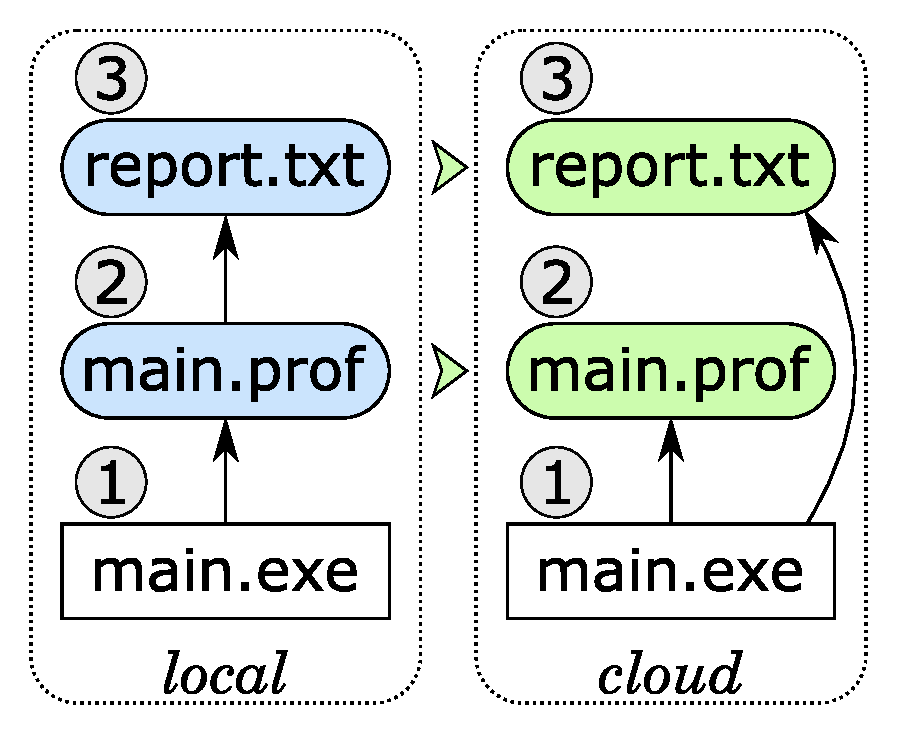
\includegraphics[scale=0.26]{fig/frankenbuild-example-build.pdf}}
% \vspace{-1.5mm}
\caption{Initial build}
\end{subfigure}
\begin{subfigure}[b]{0.31\linewidth}
\centerline{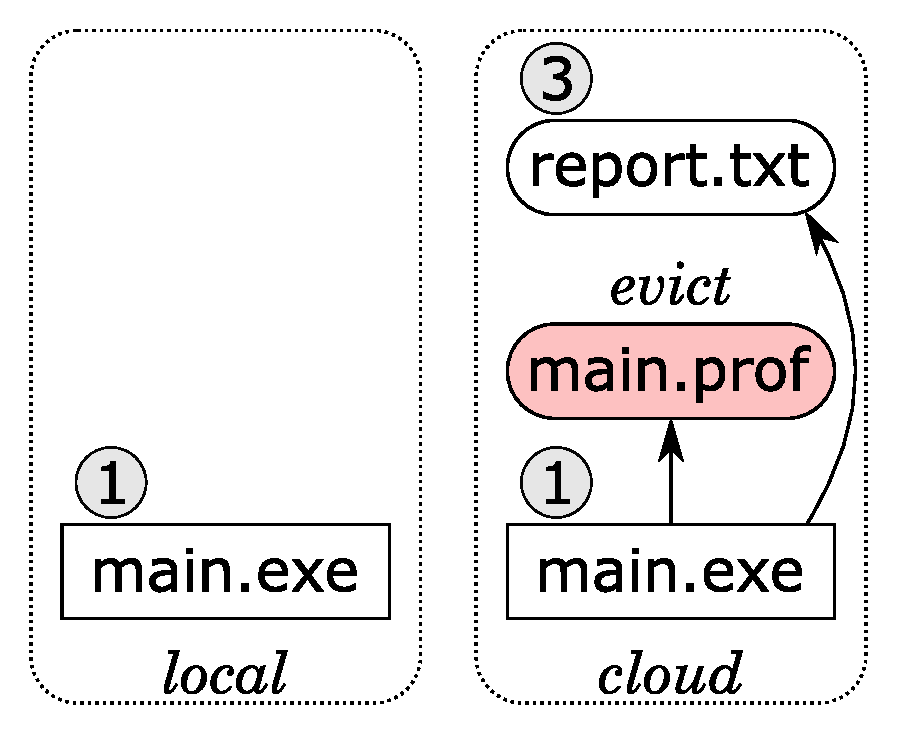
\includegraphics[scale=0.26]{fig/frankenbuild-example-clean.pdf}}
% \vspace{-1.5mm}
\caption{Clean up, evict \cmd{main.prof}}
\end{subfigure}
\begin{subfigure}[b]{0.36\linewidth}
\centerline{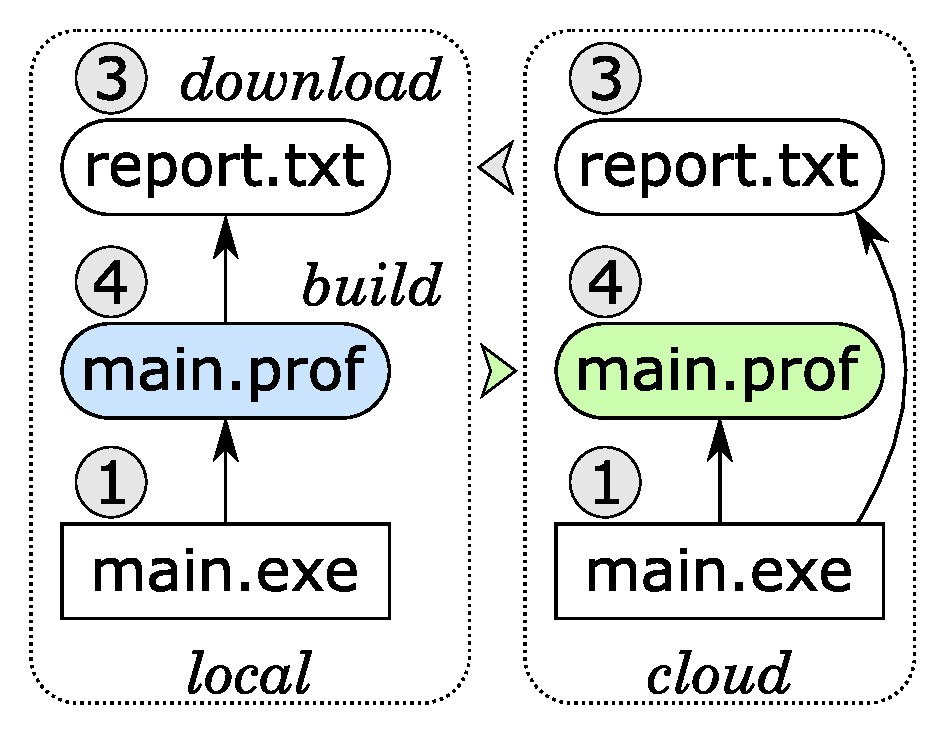
\includegraphics[scale=0.26]{fig/frankenbuild-example-rebuild.pdf}}
% \vspace{-1.5mm}
\caption{Build \cmd{main.prof} and \cmd{report.txt}}
\end{subfigure}
% \vspace{-1.5mm}
\caption{A Frankenbuild example: (a)~build a human-readable profiling report for
\cmd{main.exe} from information dump \cmd{main.prof} produced by a profiling
tool, then record deep constructive traces in the cloud, (b)~remove built files
locally and evict \cmd{main.prof} from the cloud storage, (c)~build
\cmd{main.prof} by executing the profiler (profiling is non-deterministic, hence
the new hash value), then build \cmd{report.txt} by downloading it from the
matching deep constructive trace in the cloud, resulting in a Frankenbuild
because \cmd{main.prof} and \cmd{report.txt} are inconsistent. New and evicted
cloud storage entries are highlighted; file hashes are shown in circles.
\label{fig-frankenbuild}}
% \vspace{-4mm}
\end{figure}

Deep constructive traces (\S\ref{sec-deep-constructive-traces}) combined with
task non-determinism (\S\ref{sec-non-determinism}) can lead to very subtle bugs,
especially in the cloud setting. Fig.~\ref{fig-frankenbuild} shows a
\emph{Frankenbuild}~\cite{esfahani2016cloudbuild} example, where the target
\cmd{report.txt}, which is downloaded from the cloud, is inconsistent with its
immediate dependency \cmd{main.prof}. This inconsistency is caused by two factors:
(i)~inherent non-determinism of profiling: running a profiling tool on the very
same \cmd{main.exe} will produce different \cmd{main.prof} results every time;
and (ii)~relying on deep constructive traces, which cache build results based
only on the hashes of terminal task inputs (in this case \cmd{main.exe}). Note
that the resulting store is incorrect according to all three definitions of
correctness: the main definition~(\S\ref{sec-build-correctness}), the variant
for non-deterministic tasks~(\S\ref{sec-non-determinism}) and the variant for
shallow builds~(this section).

% \todo{AM/NM}{Re-using existing infrastructure: (a) key-value store, (b) remote
% execution service. Neil says: I think this is a stretch. It's a lot more nuanced
% as we saw from Bazel discussions so I'd probably skip it.}

\subsection{Iterative Computations}\label{sec-iterative-compute}

Some computations are best described not by a chain of acyclic dependencies,
but by a loop. For example, \LaTeX~requires repeated rebuilding until it
reaches a fixed point, which can be directly expressed in build systems, such as
\Pluto~\cite{erdweg2015pluto}. Another example is \Excel, where a cell can
depend on itself, for example: \cmd{A1 = A1 + 1}. In such cases \Excel will
normally not execute anything, but if the ``Iterative Calculations'' feature is
enabled \Excel will execute the formula for a specified maximum number $N$ of
times per calculation (where $N$ is a setting that defaults to 100).

For examples like \LaTeX~we consider the proper encoding to not be circular
tasks, but a series of iterative steps, as described by
Mitchell~\shortcite{shake-fixed-point}. It is important that the number of
executions is bounded, otherwise the build system may not terminate (a
legitimate concern with \LaTeX, which can be put into a situation where it is
bistable or diverging over multiple executions). The examples in \Excel tend to
encode either mutable state, or recurrence relations. The former is only
required because \Excel inherently lacks the ability to write mutable state, and
the latter is probably better solved using explicit recurrence formulae.

Overall we choose not to deal with cyclic dependencies -- a choice that most build
systems also follow. There are computation frameworks that support tasks with
cyclic dependencies under the assumption that tasks are \emph{monotonic} in a
certain sense~\cite{pottier2009lazy,radul2009propagation}.

\subsection{Polymorphic values}\label{sec-polymorphism}

Our build system abstraction assumes a \hs{k}/\hs{v} store, along with a build
system that works directly on \hs{k} and \hs{v} values. However, some build
systems provide greater flexibility, e.g. \Shake permits polymorphic keys and
values, allowing types that are stored only in the \Shake's build information.
\Shake users have remarked that polymorphism provides a much easier expression
of concepts, e.g. see~Mokhov~\etal~\shortcite{hadrian}.

As one example of richer key/value types, consider the version of
\cmd{gcc}~--~for many builds it should be a dependency. In \Shake it is possible
to define an \emph{oracle} rule as per Mitchell~\shortcite{mitchell2012shake}
whose value is the result of running \cmd{gcc -}\cmd{-version} and which is
volatile, making the \cmd{gcc} version something that can be depended upon. Of
course, provided the build can express volatile dependencies and supports
cutoff, the version number could equally be written to a file and used in a
similar way, albeit at the cost of introducing additional correctness
invariants, e.g. that the file \cmd{gcc-version.txt} does indeed contains two
dot-separated integers.

Generalised algebraic data types, or GADTs~\cite{spj2006gadts}, can be used to
extend our models to support ``typed'' build tasks. The idea is to replace
the callback \hs{fetch}~\hs{::}~\hs{k}~\hs{->}~\hs{f}~\hs{v} by its
more polymorphic equivalent \hs{fetch}~\hs{::}~\hs{k}~\hs{v}~\hs{->}~\hs{f}~\hs{v},
where~\hs{k}~\hs{v} is a GADT representing keys tagged by the type~\hs{v} of
corresponding values. The idea is best explained by way of an example:

\vspace{1mm}
\begin{minted}[xleftmargin=10pt]{haskell}
data Version = Version { major :: Int, minor :: Int }
    deriving (Eq, Ord)

data Key a where
    File       :: FilePath -> Key String
    GccVersion :: Key Version
\end{minted}
\vspace{1mm}

\noindent
Here we extend the usual mapping from file paths to file contents with an
additional key type \hs{GccVersion} mapped to a \hs{Version}. The task
abstraction needs to be adjusted to cope with such keys (the suffix \hs{T}
stands for ``typed''):

\vspace{1mm}
\begin{minted}[xleftmargin=10pt]{haskell}
type Fetch k f = @\std{forall}@ v. k v -> f v

newtype TaskT c k v = TaskT { runT :: @\std{forall}@ f. c f => Fetch k f -> f v }

type TasksT c k = @\std{forall}@ v. k v -> Maybe (TaskT c k v)
\end{minted}
\vspace{1mm}

\noindent
The changes compared to the definition in~\S\ref{sec-task} are minimal: (i) the
\hs{TaskT} now uses a typed \hs{Fetch} callback (we define a separate type
synonym only for readability), and (ii) the type of \hs{TasksT} is now
polymorphic in \hs{v} instead of being parameterised by a concrete \hs{v}. The
example below demonstrates how \hs{fetch} can be used to retrieve dependencies
of different types: the rule \cmd{release.txt} concatenates the contents of two
\hs{File}s, while the rule \cmd{main.o} uses the numeric \hs{GccVersion} to
determine the way the \hs{source} file should be compiled.

\vspace{1mm}
\begin{minted}[xleftmargin=10pt]{haskell}
example :: TasksT Monad Key
example (File "release.txt") = Just $ TaskT $ \fetch -> do
    readme  <- fetch (File "README")
    license <- fetch (File "LICENSE")
    return (readme ++ license)
example (File "main.o") = Just $ TaskT $ \fetch -> do
    let source = "main.c"
    version <- fetch GccVersion
    if version >= Version 8 0 then compileNew source
                              else compileOld source
example _ = Nothing
\end{minted}
\vspace{1mm}

\subsection{Multiple-Output Build Tasks}\label{sec-multiple-outputs}

We can use the extra polymorphism from \S\ref{sec-polymorphism} for build tasks that produce multiple output
keys~--~for example, \cmd{ghc A.hs} produces both \cmd{A.hi} and \cmd{A.o}.
That can be represented by having a key whose value is a pair of file names, and
whose result is a pair of file contents. From that, the task for \cmd{A.hi}
can be the first component of the result of the pair. Such an operation
can be encoded without polymorphic keys provided the pair of files (or a dummy
file representing the pair) is marked as changed if either of the contained
files change, but it is more elegant and type-safe with the extra polymorphism.

Multiple-output build tasks require one more convenience mechanism,
which is orthogonal to polymorphism. Multiple-output task descriptions partition
the set of keys into \emph{elementary subsets} e.g.
$\{\cmd{A.hi},\cmd{A.o}\} \rightarrow \cmd{ghcTask}$,
$\{\cmd{B.o}\} \rightarrow \cmd{gccTask}$, etc. It is very convenient to
allow to fetch arbitrary sets of keys, such as $\{\cmd{A.o},\cmd{B.o}\}$,
without manually decomposing them into appropriate elementary subsets. This
requires a method to efficiently construct task descriptions operating on
arbitrary sets of keys rather on elementary subsets. One way to implement such
``multiple-output task closure'' is shown below.

\vspace{1mm}
\begin{minted}[xleftmargin=10pt]{haskell}
type Partition k = k -> [k]

multi :: Eq k => Partition k -> Tasks Applicative [k] [v]
                             -> Tasks Applicative [k] [v]
multi partition tasks keys
    | k:_ <- keys, partition k == keys = tasks keys
    | otherwise = Just $ Task $ \fetch ->
        sequenceA [ select k <$> fetch (partition k) | k <- keys ]
  where
    select k = fromMaybe (error msg) . lookup k . zip (partition k)
    msg = "Partition invariants violated"
\end{minted}
\vspace{1mm}

\noindent
The function \hs{multi} takes a task description \hs{tasks} that operates on
elementary key subsets, and computes its closure supporting all possible
combinations of keys. The first argument \hs{partition} specifies the elementary
key subsets supported by the original \hs{tasks}. There are two cases: (i) if a
given set of \hs{keys} is an elementary subset, we pass the query to \hs{tasks};
(ii) otherwise, we examine every key \hs{k} in \hs{keys}, \hs{fetch} its
corresponding elementary subset, and \hs{select} the appropriate value from the
result. Returning to the above example, when given the query
$\{\cmd{A.o},\cmd{B.o}\}$, this function will \hs{fetch} elementary subsets
$\{\cmd{A.hi},\cmd{A.o}\}$ and $\{\cmd{B.o}\}$, thereby depending on the
corresponding build tasks \cmd{ghcTask} and \cmd{gccTask}.

We chose not to use polymorphic tasks in the above implementation for
simplicity, but nothing prevents us from combining polymorphism with
multiple-output task closure.

% \todo{AM/NM}{We are talking about sets above, but are using lists, which is a
% bit inconsistent. We could switch from \hs{[k]} to \hs{Set k} fairly easily.
% Shall we? Neil says: Haskell code dealing with sets is quite a lot more complex.
% People are used to being quite fuzzy around the difference - I'd leave it as is.
% Andrey says: Also, using \hs{Set v} doesn't seem possible, because we won't be
% able to relate \hs{v}s with corresponding \hs{k}s}.

\subsection{Self-tracking}\label{sec-tracking-aspects}

Some build systems, for example \Excel and \Ninja, are capable of recomputing a
task if either its dependencies change, \emph{or} the task itself changes. For
example:

\vspace{0.5mm}
\begin{minted}[xleftmargin=10pt]{text}
A1 = 20      B1 = A1 + A2
A2 = 10
\end{minted}
\vspace{0.5mm}

\noindent
In \Excel the user can alter the value produced by \cmd{B1} by either editing
the inputs of \cmd{A1} or \cmd{A2}, \emph{or} editing the formula in
\cmd{B1}~--~e.g. to \cmd{A1 * A2}. This pattern can be captured by describing
the rule producing \cmd{B1} as also depending on the value \cmd{B1-formula}.
The implementation can be given very directly in a
\hs{Tasks}~\hs{Monad}~--~concretely, first look up the formula, then interpret
it:

\vspace{1mm}
\begin{minted}[xleftmargin=10pt]{haskell}
sprsh4 "B1" = Just $ Task $ \fetch -> do
    formula <- fetch "B1-formula"
    evalFormula fetch formula
\end{minted}
\vspace{1mm}

\noindent
The build systems that have precise self-tracking are all ones which use a
\emph{non-embedded domain specific language} to describe build tasks. Those
which use a full programming language, e.g. \Shake, are faced with the challenge
of implementing equality on arbitrary task functions. For such build systems,
the pessimistic assumption that any change to the build system potentially
changes any build task can often be used~--~the classic example being a makefile
depending on itself.

Below we show how to implement self-tracking in a build system that allows users
to describe build tasks by \emph{scripts} written in a non-embedded domain
specific language. We will denote the type of scripts by \hs{s}, and will assume
that scripts are indexed by keys \hs{k} just like all other values \hs{v}. More
specifically, we use the following GADT to tag keys \hs{k} with corresponding
result types: \hs{s} for scripts, and \hs{v} for other values.

\vspace{1mm}
\begin{minted}[xleftmargin=10pt]{haskell}
data Key k v s a where
    Script :: k -> Key k v s s -- Keys for build scripts
    Value  :: k -> Key k v s v -- Keys for all other values
\end{minted}
\vspace{1mm}

\noindent
The function \hs{selfTracking} defined below is a generalisation of the approach
explained in the above \Excel example \hs{sprsh4}. The function takes a parser
for scripts, of type \hs{s}~\hs{->}~\hs{Task}~\hs{Monad}~\hs{k}~\hs{v}, and a
description of \emph{how to build all scripts}, of type
\hs{Tasks}~\hs{Monad}~\hs{k}~\hs{s}. For \hs{sprsh4}, the latter would simply
fetch \cmd{B1-formula} when given the key \cmd{B1} and return \hs{Nothing}
otherwise, but the presented approach can cope with much more sophisticated
scenarios where scripts themselves are derived from ``script sources'', e.g. all
C compilation scripts can be obtained from a single pattern rule, such as
\cmd{gcc -c [source] -o [object]}. The resulting typed task description
\hs{TasksT}~\hs{Monad}~\hs{(Key}~\hs{k}~\hs{v}~\hs{s)} tracks both values and
scripts that compute them, and is therefore self-tracking.

\vspace{1mm}
\begin{minted}[xleftmargin=10pt]{haskell}
selfTracking :: (s -> Task Monad k v) -> Tasks Monad k s
                                      -> TasksT Monad (Key k v s)
selfTracking _     _     (Script _) = Nothing -- Scripts are inputs
selfTracking parse tasks (Value  k) = runScript <$> tasks k
  where
    -- Fetch the script, parse it, and then run the obtained task
    runScript :: Task Monad k s -> TaskT Monad (Key k v s) v
    runScript task = TaskT $ \fetch -> do
        script <- run task (fetch . Script)
        run (parse script) (fetch . Value)
\end{minted}
\vspace{1mm}

\noindent
It is possible to implement \hs{selfTracking} without relying on GADTs and typed
tasks presented in~\S\ref{sec-polymorphism}, at the cost of using partial
functions.
